\section*{Assignment 5}
% Password.
% Fpga was counting time ow long the responsetime was for responding, waiting for the 1st didgit of the answere. middelng the time between als answeres to get the longes one right. using thatone as correct didgit of the PW.
%
% building the counter 4 the clockcycles was the hard part strings where to long
% fpga giving back the time  we had to use 2 bytes
% 
% python did the rest.

Like in assignment 4, we get get a microcontroller (this time we know, that its sowftware is written in c) and analyse it the same way. 
This time it directly prompts \textit{``Please enter password''} and the goal is set. As possible attack vector comes a timing vulnerability to mind, if the password comparison is implemented using \texttt{strcmp}. We continue setting up the FPGA like before -- able to reset the device on command and relaying all communication. We just need a little further testing to know, that we are indeed going to program a timing attack.

Bruteforce attack against password string. 

See figure \ref{fig:as5-schematic} (p.~\pageref{fig:as5-schematic}).

\begin{figure}[tb]
    \begin{center}
        \usetikzlibrary{arrows.meta}
\usetikzlibrary{calc,intersections,through,backgrounds}
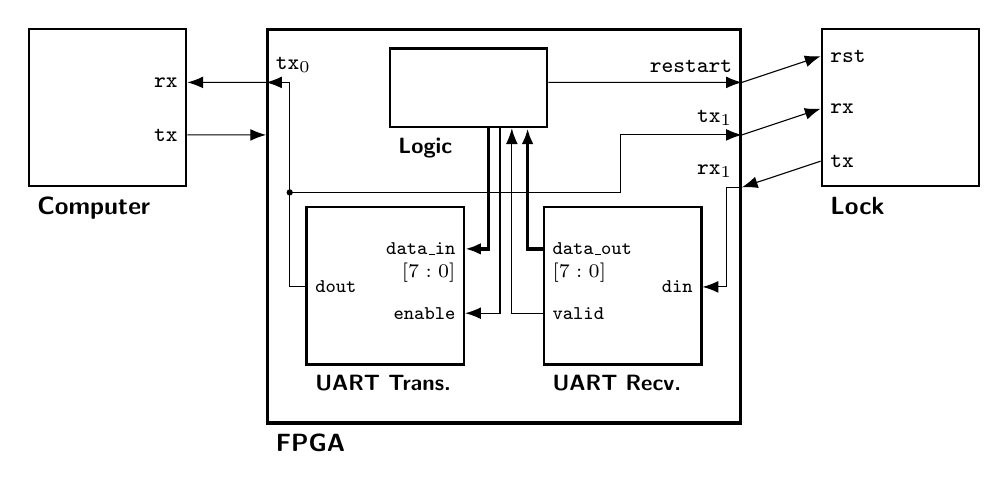
\begin{tikzpicture}
% 	\tikzset{
% 	  every node/.style={scale=1.1}
% 	}	
	\tikzset{comp/.style={
		rectangle, draw=black, thick
	}}	
	\tikzset{component/.style={
		comp, minimum width=6cm, minimum height=5cm, very thick
	}}
	\tikzset{component_small/.style={
		comp, minimum width=2cm, minimum height=2cm, thick
	}}
	\tikzset{caption/.style={
		below right
	}}
	\tikzset{conn/.style={
		-{Latex[length=2mm]}
	}}
	
	% FPGA
	\node (FPGA) [component] at (0,0) {}
		% Caption
		node [caption] at (FPGA.south west) { \small{\textsf{\textbf{FPGA}}} }
		
		% In/-outputs links
		coordinate [yshift=3cm+0.4pt+0.666cm, label={ above right : \footnotesize{} }]                           (FPGA_rx0) at (FPGA.south west) % unten
		coordinate [yshift=3cm+0.4pt+1.333cm, label={ above right : \footnotesize{$\texttt{tx}_0$} }] (FPGA_tx0) at (FPGA.south west) % oben

		% In/outputs  rechts
		coordinate [yshift=3cm+0.4pt,                    label={ above left : \footnotesize{$\texttt{rx}_1$} }]      (FPGA_rx1)       at (FPGA.south east)  % unten
		coordinate [yshift=3cm+0.4pt+0.666cm, label={ above left : \footnotesize{$\texttt{tx}_1$} }]      (FPGA_tx1)       at (FPGA.south east) % mitte
		coordinate [yshift=3cm+0.4pt+1.333cm, label={ above left : \footnotesize{$\texttt{restart}$} }] (FPGA_restart) at (FPGA.south east) % oben
	;

	% Logic
	\node (Logic) at (FPGA.north) [comp, minimum height=1cm, minimum width=2cm, below, shift={(-0.45cm, -0.25cm)}] {}
		node [caption] at (Logic.south west) { \textsf{\footnotesize{\textbf{Logic}}} }
	;

	% Receiver
	\node (Receiver) at (FPGA.south east) [component_small, above left, shift={(-0.5, 0.75)}] {}
		% Caption
		node [caption] at (Receiver.south west) { \textsf{\footnotesize{\textbf{UART Recv.}}} }

		% Input rechts
		coordinate [yshift=1cm, label={ left : \scriptsize{\texttt{din}} }] (Receiver_din) at (Receiver.south east)

		% Outpus links
		coordinate [yshift=0.666cm,                 label={ right : \scriptsize{\texttt{valid}} }]           (Receiver_valid)           at (Receiver.south west) % unten
		coordinate [yshift=1.333cm+0.15cm, label={ right : \scriptsize{\texttt{data\_out}} }] (Receiver_data_out)    at (Receiver.south west) % oben
		coordinate [yshift=1.333cm-0.15cm,  label={ right : \scriptsize{$[7:0]$} }]                     (Receiver_data_out2) at (Receiver.south west) % mitte
	;

	% Transmitter
	\node (Transmitter) at (FPGA.south west) [component_small, above right, shift={(0.5, 0.75)}] {}
		node [caption] at (Transmitter.south west) { \textsf{\footnotesize{\textbf{UART Trans.}}} }

		% Output links
		coordinate [yshift=1cm, label={ right: \scriptsize{\textsf{\texttt{dout}}} }] (Transmitter_dout) at (Transmitter.south west) % unten

		% Inputs links
		coordinate [yshift=0.666cm,                 label={ left : \scriptsize{\texttt{enable}} }]    (Transmitter_enable)   at (Transmitter.south east) % unten
		coordinate [yshift=1.333cm-0.15cm,  label={ left : \scriptsize{$[7:0]$} }]                  (Transmitter_data_in2)at (Transmitter.south east) % mitte
		coordinate [yshift=1.333cm+0.15cm, label={ left : \scriptsize{\texttt{data\_in}} }] (Transmitter_data_in)  at (Transmitter.south east) % oben	
	;

	% Computer
	\node (Computer) [component_small, below left, xshift=-1cm] at (FPGA.north west) {}
		% Caption
		node [caption] at (Computer.south west) { \small{\textsf{\textbf{Computer}}} }

		% In/outputs rechts
		coordinate [yshift=0.666cm, label={ left:\footnotesize{\texttt{tx}} }] (Computer_tx) at (Computer.south east) % unten
		coordinate [yshift=1.333cm, label={ left:\footnotesize{\texttt{rx}} }] (Computer_rx) at (Computer.south east) % oben
	;

	% Lock
	\node (Lock) [component_small, below right, xshift=1cm] at (FPGA.north east) {}
		% Caption
		node [caption] at (Lock.south west) { \small{\textsf{\textbf{Lock}}} }

		% In/outputs rechts
		coordinate [yshift=0.333cm, label={ right:\footnotesize{\texttt{tx}} }]   (Lock_tx)   at (Lock.south west) % unten
		coordinate [yshift=0.999cm, label={ right:\footnotesize{\texttt{rx}} }]   (Lock_rx)   at (Lock.south west) % mitte
		coordinate [yshift=1.666cm, label={ right:\footnotesize{\texttt{rst}} }] (Lock_rst)  at (Lock.south west) % oben
	;

	% Computer <-> FPGA
	\draw[conn]  (FPGA_tx0) -- (Computer_rx);
	\draw[conn] (Computer_tx) -- (FPGA_rx0);

	% FPGA <-> Lock
	\draw[conn] (FPGA_restart) -- (Lock_rst);
	\draw[conn] (FPGA_tx1) -- (Lock_rx);
	\draw[conn] (Lock_tx) -- (FPGA_rx1) ;
	
	% FPGA internal
		\draw[conn] ([yshift=0.583cm] Logic.south east) -- (FPGA_restart);
	
		% Connections to/from Receiver
		\draw[conn] (FPGA_rx1) -- ([xshift=-0.2cm] FPGA_rx1) |- (Receiver_din);
		\draw[conn, very thick] (Receiver_data_out) -| ([xshift=0.75cm] Logic.south); 
		\draw[conn] (Receiver_valid) -| ([xshift=0.55cm] Logic.south);
		
		% Connections to/from Transmitter
		\draw[conn, very thick] ([xshift=0.25cm]Logic.south) |- (Transmitter_data_in);
		\draw[conn] ([xshift=0.4cm] Logic.south) |- (Transmitter_enable);
		\draw[conn, name path=Transmitter_dout--FPGA_tx0] (Transmitter_dout) -- ([xshift=-0.2cm] Transmitter_dout) |- (FPGA_tx0);
		\draw[conn, name path=Transmitter_dout--FPGA_tx1] ([shift={(-0.2cm, 1.2cm)}] Transmitter_dout) -- ([shift={(4cm, 1.2cm)}] Transmitter_dout) |- (FPGA_tx1);

		% Intersection
		\fill[name intersections={of=Transmitter_dout--FPGA_tx0 and Transmitter_dout--FPGA_tx1, total=\t}] (intersection-\t) circle (0.4mm);
\end{tikzpicture}
        \caption{Timing attack.}
        \label{fig:as5-schematic}
        \vspace{1em}\hrule
    \end{center}
\end{figure}
